\newpage
\newpage
\section{Introduction}\label{introduction}

Making coffee is a part of most people's daily life. Some need it to get
going in the morning, others meet in the afternoon and enjoy it in
company.

People use it on any occasion as a reason to take a break. Just like
there are different occasions to drink coffee, there are different
methods to acquire it; the coffee shop next door, a vending machine or
the coffee machine in the kitchen. In an office it often occurs that
colleagues share a machine. But who is responsible for buying new beans,
the cleaning, or payment? These are tasks that no one likes to take over
voluntarily. So how exactly could a fair distribution of those
activities look like, and how are they executed most easily? This
question calls for an IT supported solution that tracks the coffee
drinker, the amount and the date, in order to balance their accounts
appropriately. Furthermore, statistical data can be collected that
ensures a fair distribution of the cleaning tasks.

Those aspects motivated us, Cornelius Pohl, Daniel Birnstiel, and
Theresa Zobel to develop a solution for the coffee machine
administration in the office in the context of the tBPM seminar, during
the summer term 2015, at the BPT chair of Professor Weske. The goal was
to create a software that could work largely autonomously and simplify
any employee's work day.

\newpage
\newpage
\section{Organisational Process}\label{organisational-process}

\subsection{General}\label{general}

Like many other software projects, we used the scrum technique for
Coffee-in-the-Cloud. That means we organised the project with Jira,
which is an issue tracking software developed by Altassian. Our main
communication tool for the team itself was Slack and Facebook messenger.
We used Slack as it provides the possibility to integrate Git
notifications and many more. We had weekly stand-up meetings and
biweekly sprints.

\subsection{Functional Requirements - User Stories}\label{functional-requirements---userstories}

All the user stories where assessed and discussed beforehand. The effort
and the core features were determined. Below the user stories are
explained in detail according to their sprints.

\subsubsection{Sprint 1}\label{sprint-1}

\subsubsection*{Add Account}

The admin can add an account to the system including the first name,
last name, email and a picture. The password will be created
automatically and sent to the user via an email. Additionally he can
activate his account through this email.

\subsubsection*{Edit Account}

When the user is logged in, he is able to do some changes. This includes
the email address, the password and the profile picture.

\subsubsection*{Remove Account}

The admin is able to remove an account if requested.

\subsubsection*{Login}

The user can authenticate through email address and password.

\subsubsection*{Picture Login}

A set of pictures will be displayed to the user on a screen. Via
clicking or touching on a picture, the user can authenticate. Next to
the picture will be the name of the user.

\subsubsection*{Coffee Tracking}

When logged in, the user can add one or more coffees. He can undo this
action within a limited time frame.

\subsubsection*{Cleaning Schedule}

The user can see the cleaning schedule for the upcomming weeks.

\subsubsection{Sprint 2}\label{sprint-2}

\subsubsection*{Email Reminder - Cleaning}

When a user is assigned for cleaning he will get an email reminder. This
reminder can be turned off in his personal settings.

\subsubsection*{Email Reminder - Account Balance}

When the user's balance goes below a certain amount he is notified via
email. This reminder can be turned off in his personal settings.

\subsubsection*{Email Confirmation - Coffee Tracking}

When tracking coffee(s) the user gets a notification via email if he
choses to. Using this email he can also undo the tracking within a
certain time frame.

\subsubsection*{Statistics}

The statistics will be generated from all data gathered. The user can
opt out of having his data displayed to others.

\subsubsection*{Checklist: Cleaning}

A checklist provided on the tablet and mobile application helps the user
to keep track of each step involved in the cleaning process.

\subsubsection*{Tutorials: Photo}

To support the processes of cleaning and coffee making a photo tutorial
is provided.

\subsubsection{Sprint 3}\label{sprint-3}

\subsubsection*{Cleaning Schedule: Intelligent Assignment}

The user responsible for cleaning is chosen by the system. It will take
into account if somebody has marked himself as absent for a certain
period of time.

\subsubsection*{Guest Account}

For tracking coffees a guest account exists. It allows guests of the
chair to also track their coffees without having their own account.

\begin{itemize}
\item The account should be accessible by the admin (login with admin credentials).
\item It should behave like a normal user account, e.g. it includes statistics.
\item This account can be enabled or disabled by system administrators.
\item A summary email should be send to the admin every X days (configurable).
\end{itemize}

\subsubsection*{User Rankings}

Rankings show some kind of leaderboard according to the amount of coffee
consumed by each user in a certain time frame. Users can opt out of
having their data displayed.

\subsubsection*{Display total amount of money available}

As an administrator I want to see how much money is available for buying
coffee. This should be shown in the admin backend. When new coffee is
bought the admin needs to reduce the total amount.

\subsubsection*{Add cleaning checklist to tablet mode}

The user wants to see the cleaning checklist even when he is not logged
in.

\subsubsection*{Distinguish between weekly and bi-weekly cleaning in calender}

As a user I want to see which kind of cleaning I should perform. The
types should be easy to distinguish, for example by color.

\subsubsection*{Show a message on the main page if selected for cleaning}

As a user I want to see whether or not I have to clean today. This
should be visible on the tablet as well as on the user page.

\subsubsection*{Settings page for users}

As a user I want to be able to configure my account on a settings page.

\begin{itemize}
\item email configuration
\item profile picture
\item password
\end{itemize}

\subsubsection*{Extend cleaning checklist}

Add restart button and finish button to the coffee checklist. Cross out
finished tasks.

\subsubsection*{Include calender entry invitation in cleaning email}

As a user I want a calendar invitation to be included in the email that
informs me about my upcoming cleanings.

\subsubsection*{Blame feature}

I want to have a feature in tablet mode to blame someone who did not
clean the porta filter. A ``reminder'' email is sent to the last coffee
drinker (add something like ``it might be possible that someone else did
not clean but did not register the coffee'').

\subsection{XP-Techniques}\label{xp-techniques}

In order to work efficiently and fulfil our users requirements as good
as possible, we used some of the practices of extreme programming. In
our opinion these helped us improve the development workflow.

\subsubsection{small releases}\label{small-releases}

We integrated code early and steadily. As a result we had less bugs and
always a running version of our software. Additionally we got the
feedback quicker and it also increased our self confidence.

\subsubsection{pair programming}\label{pair-programming}

In the course of the weeks we realized, that we did much better work
when developing together. Therefore we often implemented user stories in
pairs where one was the driver (types code) and the partner tried to be
completely engaged and provide additional thoughts.

\subsubsection{collective code ownership}\label{collective-code-ownership}

As we often worked together on user stories, everybody was allowed to
change the code of the others. This was reasonable because it avoids
expert knowledge.

\newpage
\newpage
\section{AngularJs}\label{angularjs}

In the Coffee in the Cloud-Application we use AnuglarJs for our frontend
and user interface. AnuglarJs is a Javascript framework that allows the
creation of MVC (Model-View-Controller) based web applications. Because
of this the code will stay properly divided into the three core parts
that are described below.

\begin{figure}[htbp]
\centering
\makebox[\textwidth]{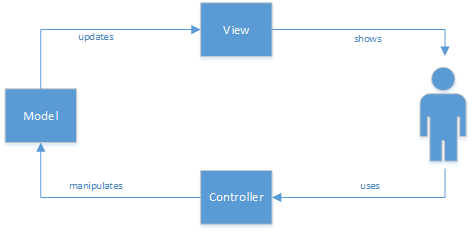
\includegraphics[width=\textwidth]{../images/mvc.png}}
\caption{mvc architecture}
\end{figure}

In order to manage dependencies we use the node package manager (short
npm) and bower. These allow installing of dependencies in a bulk.
Because of this we do not have to ship them and can keep the code base
clear.

The application loads all dependencies asynchronously through require.js
whenever they are needed. Because of this we have short loading times
and can make sure that everything is loaded in the right order.
Require.js also provides dependency injection so we do not have to worry
about initializing controllers and services ourselves.

As we do not want the application to reload every time the user performs
an action we use a routing system. This allows us to have multiple views
within one application that are loaded dynamically.

\subsection{Models}\label{models}

Models contain all kind of data we would like to use, for example users,
tally list or calendar entries. In our application these are created and
managed server-sided. The server also handles persisting the data into
our database. Because of this the models are replaced by a service that
fetches data from our server.

\subsection{Controllers}\label{controllers}

Controllers are necessary to create useful data from the stored models.
For every page that will ultimately be displayed in our application a
controller fetches the data and prepares it for the user. This also
includes validation of the user generated information.

The controllers will be both implemented server- and client-sided as
they will manage the connection between these to parts of our
application.

\subsection{Views}\label{views}

Views are responsible for displaying all data to the user. In the views
we create a user interface that will be displayed in the client's
browser. AngularJs extends the HTMl syntax and functionality to allow
the creation of basic templates in these views.

Each view is tied to a controller that determines its behaviour.

\subsection{Directives}\label{directives}

AngularJs offers a way to extend basic HTML. These so called directives
introduce new tags or attributes.

\subsection{Project structure}\label{project-structure}

The client project contains of several type of resources that are
separated in different folders.

\begin{description}
\item[/index.html] contains the main application and entry point.
\item[/js/] contains controllers, directives, services and libraries installed by bower.
\item[/less/] contains less stylesheets that will be compiled to css on deployment.
\item[/public/] contains static images and stylesheets.
\item[/views/] contains views as HTML files.
\end{description}

All other files in the client directory are resource files needed for
bower and node to include all needed dependencies.

\newpage
\newpage
\section{Finding a backend framework}\label{finding-a-backend-framework}

As our application needed a web service to run permanently we first had
to decide on a framework. We narrowed down our options to three
different technologies some of us had already worked with.

\subsection{Flask}\label{flask}

Flask is a lightweight framework for creating web services written in
Python. It offers basic routing and has nearly no overhead. While it is
very easy to use it only provides very basic functionality and thus we
would have to implement many core features like session management or
database-models ourselves. Also flask has no strict project structure
which could lead to an unstructured code base if not maintained
properly. Because we didn't want to take this risk we decided against
the flask framework.

\subsection{node.js}\label{node.js}

Node.js is a powerful framework for creating web services written in
Javascript. As we were using node.js' package manager for managing our
frontend dependencies it seemed natural to use node.js for our backend
as well. The downside was that none of us had already built a more
complex platform using it, so we would have had to slowly learn all
necessary features. We also had no knowledge of available APIs and
functionality which means we would have had to familiarize ourselves
with these before actually starting to develop our app.

\subsection{Django}\label{django}

Django is a web framework also written in Python. It has a more complex
structure but includes a lot of additional functionality, which we would
not have to implement ourselves. The core features we rely on are the
session management, the object-relationship-management for creating our
database and the url-routing for the API endpoints.

We had some experience in working with django from previous projects and
it fit our requirements perfectly.

In addition to django we are using the \texttt{rest\_framework} library
to ease the creation of a restful API. This framework provides features
to automatically create endpoints from models, data serialisation and
validation.

\newpage
\newpage
\section{Django - a short
introduction}\label{django---a-short-introduction}

A django project consists of several modules, which are thematically
separated. Each module contains models, views and other classes needed.

Django follows the MVC architecture, separating data, logic and display.
Because of this it is possible to develop logic and interface separately
from each other and maintain a clean project structure.

\subsection{Models}\label{models-1}

A model is a class that describes the data structure of objects.
Instances of these models are automatically stored into and loaded from
our database. Also changes are automatically tracked and can be reverted
at any time.

Models are defined in each module within a \texttt{models.py} file. This
file then contains one class for each model. In general these are a
subclass of the type \texttt{django.db.models.Model} and define all
fields as python data types. In addition to simple data types like
numbers and text, django also provides complex data types like dates or
files which are automatically validated. It supports all features that
are important for a relational database.

Apart from fields a model can also specify special behaviour, for example
for automatic validation when editing field values or relationships
between models.

\subsection{Permissions}\label{permissions}

A permission allows access restriction based on users and groups. The
built in permissions can be extended to allow custom control. These can
then be assigned to specific users or user groups.

Permissions can be set automatically by the system or through the
administration interface.

\subsection{Views}\label{views-1}

A view is responsible for converting model data into viewable
information. In our case each view either loads models from the database
and converts then into a JSON response or processes a request and
changes a model's state. We separated our AngularJs frontend from the
backend so our views will only represent the needed API endpoints and
will not create viewable HTML.

As we are using the \texttt{rest\_framework} extension we do not have to
handle json conversion and object validation ourselves. In this way each
view can define different methods for viewing or manipulating data.

For example a \texttt{list} method allows automatic rendering of an
object list. \texttt{post} and \texttt{get} respectively handle POST and
GET requests via the HTTP protocol.

The \texttt{rest\_framework} also provides some debugging utility. For
example when accessing an endpoint directly it displays additional
information like available methods and allows drafting new requests.
Apart from testing purposes this can also be used as a developer
documentation.

\begin{figure}[htbp]
\centering
\makebox[\textwidth]{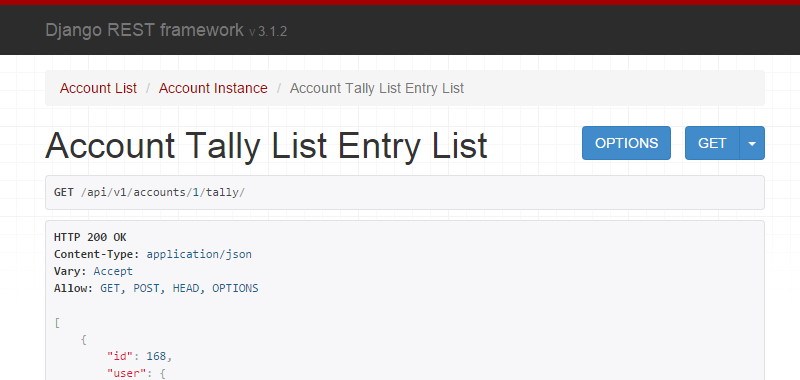
\includegraphics[width=\textwidth]{../images/rest-framework-debug.png}}
\caption{API endpoint when opened in a web browser}
\end{figure}

In order to grant an application access to a newly created view it has
to be registered in the routing system. This can be found in the
\texttt{urls.py} file and lists all
API endpoints available.

\subsection{Serializers}\label{serializers}

A serializer is responsible for converting a model into a JSON
representation. In most cases it defines a collection of fields that are
publicly accessible. For special cases like account creation it is
possible to add custom validation behaviour, which in this example
validates the password and then updates the session information.

\subsection{Migrations}\label{migrations}

Migrations are a powerful tool to alter models without manually changing
the database structure. They can be created automatically by django
after a model has been changed. It also allows for multiple developers
to change the models and then merge all changes. For example when a new
field is added to a model the author can define a default value to be
set when an existing database is upgraded. In some cases this is
necessary to not break any existing validation constraints.

A new migration can be created through the server console via the
\texttt{manage.py\ makemigrations} command. Afterwards all pending
migrations can be applied by using \texttt{manage.py\ migrate}. This
step is not necessary when creating a new database as django
automatically applies the needed changes.

\subsection{Management/Commands}\label{managementcommands}

Each module can define special commands to be used from the management
console (\texttt{manage.py}). These in general are used for
administration purposes and can only be accessed from the server side.
In our application this is used for handling automatic schedule
assignment.

Commands can be used to run a special task periodically by connecting
them with a scheduling tool like crontab.

\subsection{Templates}\label{templates}

A template contains formatted text that can be dynamically filled with
information. Usually these are used for creating dynamic HTML responses,
in our application we only use them for the email functionality.

\subsection{Static file deployment}\label{static-file-deployment}

In our application we use django to deploy all static files including
our AngularJs app. Because of this there is no need for a secondary web
server like apache. Any request that does not match a defined endpoint
will be resolved within a given directory which is specified inside the
server configuration.

\subsection{Settings}\label{settings}

To configure the server django provides a configuration file which can
be found at \texttt{/server/server/settings.py} file. The most important settings are

\begin{description}
\item[INSTALLED\_APPS] A list of installed modules and frameworks in
this application. When a new module is created it has to be added to
this list manually.

\item[DATABASES] A list of available databases that can be accessed
by the application. By default an sqlite3 connection is configured here.

\item[LANGUAGE\_CODE, TIME\_ZONE] This setting provides localisation
to our application. By default it is set to an English locale and the
Central European time zone.

\item[STATICFILES\_DIRS] A list of paths where django will search for
static files. For our application it is important to include the client
directory because otherwise it cannot be deployed.

\item[MEDIA\_ROOT] A directory where django will store uploaded files
which should be given as an absolute path. This directory has to be
writeable because otherwise any uploads will fail.

\item[DEBUG] This settings enables extended error messages. It is
helpful for testing the application but should not be used in a
productive environment.
\end{description}

\subsection{Custom settings}\label{custom-settings}

Apart from default settings we use the configuration file to add our own
options.

\begin{description}
\item[AUTH\_USER\_MODEL] Name of the desired user model. In our
application we use an own model which includes additional fields.

\item[COFFEE\_PRICE] The price of a single coffee in euros.

\item[MAIL\_SERVER, MAIL\_SENDER] Email configuration for
notifications, set to the HPI server by default.
\end{description}

\subsection{Administration interface}\label{administration-interface}

Django provides an administration interface which allows all users
tagged as \texttt{staff} to manipulate models directly. This can be used
to correct errors or create objects manually. Every action taken in the
administration interface will be logged in case some unwanted changes
are made.

A common usage would be to change a user's password, in case they forgot
it.

\begin{figure}[htbp]
\centering
\makebox[\textwidth]{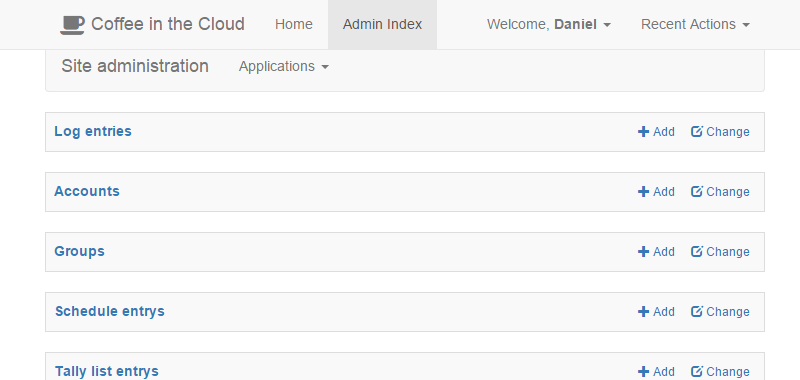
\includegraphics[width=\textwidth]{../images/django-admin.png}}
\caption{default administration view}
\end{figure}

\newpage
\newpage
\section{Architectural Overview}\label{architectural-overview}

The Coffee-in-the-Cloud application consists of a separated client and
server part. Both communicate through a common interface and will be
described in detail within the next pages.

\begin{figure}[htbp]
\centering
\makebox[\textwidth]{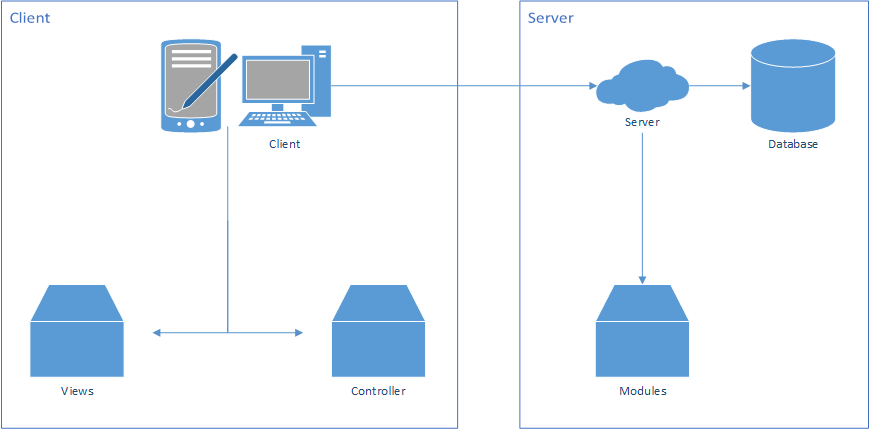
\includegraphics[width=\textwidth]{../images/architecture.png}}
\caption{architectural overview}
\end{figure}

\newpage
\newpage
\section{Frontend Architecture}\label{frontend-architecture}

The frontend for our Coffee-in-the-Cloud application is written in
Javascript using among others the AngularJs and requireJs framework as
well as bootstrap.

In the following we will explain the detailed structure of our
application's frontend.

\subsection{Services}\label{services}

As some functionality was needed on multiple occasions we grouped them
into services. This allows the functions to be available for all
controllers without having to reimplement them.

\subsubsection{coffeeCloud service}\label{coffeecloud-service}

The \texttt{coffeeCloud} service is responsible for communicating with
our backend. Each function sends a request with the desired information
to the server. All requests use the deferred API to allow chaining
actions together and enable parallel processing.

The requests are divided into these categories:

\begin{description}
\item[user] mainly provides authentication functionality and allows
querying user objects.

\item[tally] is responsible for adding or removing entries to a user's
tally list.

\item[schedule] provides functions to query the cleaning schedule.

\item[statistics] fetches relevant data for generating statistics and
preprocesses it.

\item[settings] allows fetching and storing a user's settings.

\item[balance] allows a user to manage the global balance.

\item[blame] encapsulates the blame feature.
\end{description}

\subsubsection{status service}\label{status-service}

The \texttt{status} service is responsible for displaying notifications
to the user. They are based on bootstrap alerts and are dynamically
generated. The service supports information, success, warning and error
messages.

\begin{figure}[htbp]
\centering
\makebox[\textwidth]{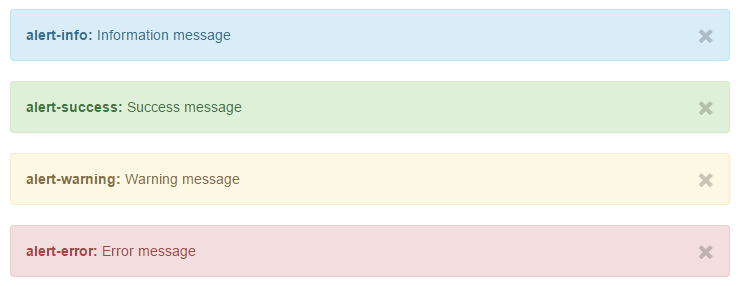
\includegraphics[width=\textwidth]{../images/service-status.png}}
\caption{list of available statuses}
\end{figure}

\subsection{Controllers and Views}\label{controllers-and-views}

\subsubsection{Main Page - Home}\label{main-page---home}

The \textbf{Main Page} is the first page seen when visiting the
coffee-in-the-cloud page. It consists of the
\texttt{welcomeController.js} and the view \texttt{welcome.html}.

\subsubsection*{welcomeController.js}

The main task of the controller is to give an alert-message saying
``Thank you for doing the cleaning!''. This happens after someone did
the cleaning and pressed the \emph{Finished Cleaning} button. In the
case that an error occurred during the function call, another alert will
tell you so.

\subsubsection*{welcome.html}

The welcome view has two states depending on whether or not you are
logged in.

\subsubsection*{\emph{Logged out}}

When first visiting the page without being logged in, you will be
greeted and have the possibility to log in via a ``sign in'' button.
Furthermore you are able to click on the tutorials and cleaning checklist
navbar tab or click on the icons for tablet mode and admin interface in
the footer.

\subsubsection*{\emph{Logged In}}

When logged in, different kind of banners can be seen. The one in blue,
which is always shown, states how many coffees you have on the list and
your current balance. If this balance is below 2.00 Euro, another red
banner appears and kindly asks you to add more money to your account. By
clicking on the x, this banner disappears.

In case you are selected for cleaning, a third banner in yellow can be
seen beneath. There you can either close the banner by clicking on the x
or tell the system, that you successfully finished the cleaning by
clicking the check. This can alternatively be done when pressing the
``finished cleaning''-Button.

Moreover, you will get complimented if you are the number one coffee
drinker. This is again shown by a blue banner stating ``You have drunk
most of the coffee so far. Good job!''. It can be closed as well. The
data used for estimating the winner, is loaded on login in the
loginController.

Of course, one has access to all the other navbar tabs like statistics
or the tally list when logged in, too.

\subsubsection{Login}\label{login}

For logging in via the login button, on the one hand the
\texttt{loginController.js} and on the other hand the
\texttt{login-popup.html} view is needed.

\subsubsection*{loginController.js}

The loginController has a lot of functionality as it loads all the
necessary data beforehand. In order to keep the code clean and avoid any
unnecessary repetitions we outsourced functions, which are called more
often by different views, in the loginController.

As mentioned in the paragraph before, the ranking is calculated here. So
every time someone logs in, the controller compares the tally list
entries of all the users and estimates the winner(s).

One of the global function in the loginController is
\emph{updateUser()}. This function is called on several occasions. For
example, when the user logs in. It is responsible for updating the
currently logged in user's data and loads the user object and his tally
list from the server. Additionally it is checked whether or not the user
is selected for cleaning.

We decided to not move this function into a separate service as it is
tied to the login process. Instead we used AngularJs' event system to
notify the controller if an update is needed.

The second global method is \emph{updateTally()}, called when you add a
coffee to your tally list.

When the user wants to logout and presses the ``sign out'' button, the
controller accomplishes the logout process by calling the
\texttt{logout()} function.

\subsubsection*{login-popup.html}

The login-popup appears when the ``sign in'' button is clicked on. The
user can now enter his login credentials consisting of an email address
and a password. By clicking ``Login'' the \texttt{login()} function is
called in the loginController. Otherwise the user can abort the login
process by simply pressing ``cancel''. Once logged in, a short alert
message welcomes the user and he now has full access to the
web-application.

\subsubsection{Tally List}\label{tally-list}

In order to see the current coffee consumption the user visits the
\emph{tally list} tab for which the \texttt{tallylistController.js}
controller and the corresponding \texttt{tallylist.html} view is
responsible.

\subsubsection*{tallylistController.js}

The \texttt{tallylistController} has two core methods. On the one hand,
when a coffee is added to the tally list the \texttt{addCoffee(amount)}
function is called. The amount depends on whether the user decides to
drink a single or a double coffee. Following this the two global methods
\texttt{updateTally()} and \texttt{updateUser()} from the
\texttt{LoginController} are notified through the event bus.

On the other hand, the user has the possibility to revise the adding
within half an hour. Therefore the \texttt{removeCoffee(id)} is called
with the matching coffee ID. This causes the entry to be removed from
the users tally list.

\subsubsection*{tallylist.html}

Like on the main page the user is shown a banner with his current
balance and the amount of coffees on the list. Additionally, if the
balance is low, a warning appears.

The user now has the possibility to add a single or a double coffee to
his tally list by pressing the corresponding button. This will trigger
the \texttt{addCoffee(amount)} function in the
\texttt{tallylistContoller}. Of course, after adding the coffee, the
banners are updated with the new amount of coffees and balance.

As mentioned beforehand the user is able to revise the adding of the
coffee by clicking on the bin symbol. This is only possible within the
next half hour of adding.

\subsubsection{Cleaning Schedule}\label{cleaning-schedule}

As the cleaning of the coffee machine has to be scheduled, we built a
calendar composed of the \texttt{scheduleController.js} and the
\texttt{schedule.html}.

\subsubsection*{scheduleController.js and schedule.html}

The controller sends a request to the backend in order to receive the
necessary data for the calendar. How the algorithm works, will be
explained later on. The data important for us is the user and the type
of cleaning assigned. To distinguish between the different kinds of
cleaning we assigned them different colors. Additionally if the cleaning
is finished, it will be shown as crossed out and in gray. Of course one
can select between daily, weekly and monthly view in the calendar.

For displaying an appealing calendar we use the
\href{http://fullcalendar.io/}{fullcalendar} library.

\subsubsection{Statistics}\label{statistics}

In order to compare his own coffee consumption with the consumption of
others, we thought about some useful diagrams to show different
comparisons. In the end we came up with four kinds:

\begin{enumerate}
\def\labelenumi{\arabic{enumi}.}
\item
  the overall coffee consumption
\item
  the users coffee consumption
\item
  the amount of single and double coffee consumed
\item
  the users coffee consumption compared to the overall consumption
\end{enumerate}

The Javascript framework \href{chartjs.org/docs/}{chartJs} supplied us
with some interesting chart types we could add into our application.

\subsubsection*{statisticsController.js and statistics.html}

The procedure is rather simple. The \texttt{statisticsController} sends
a request to the backend in order to get the necessary data. Then the
data will be processed according to the requirements of the diagram
type. Consequently the diagrams are filled with the matching data.

\subsubsection{Tutorials}\label{tutorials}

The tutorials page is one of the pages, which can be seen even if the
user is not logged in. It allows the user to have a step by step
introduction to coffee making which is supported by pictures.

\subsubsection*{tutorialsController.js and tutorials.html}

The controller automatically generates the picture tutorial from a
dataset. In case the user has to make a decision different lines of
action will be pursued.

In the \texttt{tutorialsController} the important method is
\texttt{next(cb)}. It is called by clicking on the picture directly or
the arrows next to the pictures. This function then fetches the next
picture or set of pictures and displays them to the user.

\subsubsection{Cleaning Checklist}\label{cleaning-checklist}

Just like the photo tutorial shows the user how to make perfect coffee,
the cleaning checklist supports the cleaning of the machine.

\subsubsection*{cleaningController.js and cleaning-checklist.html}

In this controller all the steps required to clean the machine are
included. Now depending on weekly or biweekly cleaning the right steps
are shown to the user. He can switch between different types of cleaning
by clicking one of the provided buttons. All the steps are listed and
can be crossed out when finished. It is also possible so reset the list
and start from the beginning.

After the cleaning is done, the user can mark is cleaning duty as done
by simply pressing the \emph{Finished Cleaning} button, which is located
at the bottom of the page or at the main page. If he does so the
cleaning notification will disappear and the calendar entry will be
marked as done.

\subsubsection{Picture Login - Tablet
Mode}\label{picture-login---tablet-mode}

One of the core features required was the tablet mode. Here the user
does not need to log in with his login credentials but rather click on
his picture to add a coffee to his account.

\subsubsection*{pictureloginController.js and picture-login.html}

As the user does not login with his credentials, he has limited access
to the website. That means, he is only able to see the tutorials and the
cleaning checklist. However if someone is selected for cleaning, a
banner will tell you so.

The procedure of adding a coffee in tablet mode is nearly the same as
adding a coffee when logged in. So again after selecting the coffee size
the \texttt{updateTally()} event is dispatched.

Another feature especially implemented for the tablet mode is the blame
button. If someone clicks on this button, the person last adding a coffee
will get a blame email and a reminder to clean up the kitchen in the
future.

\subsubsection{Settings}\label{settings-1}

The Settings page has two states, deping on whether or not the user has
the permission to manage the global balance.

\subsubsection*{settings.html}

\subsubsection*{\emph{basic user}}

The user is able to change his avatar for the picture login as well as
his password. Additionally the user can decide, if he wants the data
about his coffee consumption to be evaluated in the statistics and
ranking. As receiving emails can be really annoying, we decided in favour
of an option to disable all notifications.

\subsubsection*{\emph{admin user}}

The admin has more power over the global balance and is able to add
money to users balance.

\subsubsection*{settingsController.js}

The controller contains two important methods. \texttt{update()} is
called, when the user submits his data. If he wants to change is
password he is required to enter his new password twice and the function
then validates the passwords.

Moreover, the balance of a user can be changed by the admin. If so,
\texttt{update\_balance()} is executed and shows an alert-message if it
succeeded.

\newpage
\newpage
\section{Backend Architecture}\label{backend-architecture}

The backend for our Coffee-in-the-Cloud application is written in Python
using the django web service framework.

In the current application release the following modules are used.

\subsection{database layout}\label{database-layout}

Each model is represented by a data table in our relational database.

\begin{figure}[htbp]
\centering
\makebox[\textwidth]{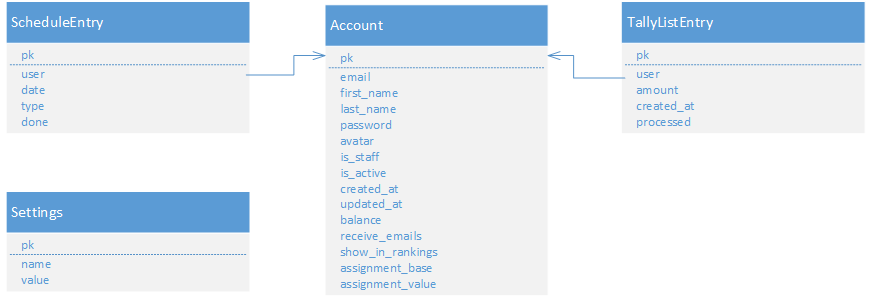
\includegraphics[width=\textwidth]{../images/class-diagram.png}}
\caption{class diagram}
\end{figure}

\subsection{authentication}\label{authentication}

The \texttt{authentication} module is responsible for user management
and extends the built-in system django uses. While django provides a
simple authentication and security system we decided to extend it in
order to allow more customization.

\subsubsection{API Endpoints}\label{api-endpoints}

\begin{description}
\item[\texttt{GET\ /api/v1/accounts/}] Query a list of all registered accounts.

\item[\texttt{GET\ /api/v1/accounts/\{ID\}/}] Query an account specified by
\{ID\}.

\item[\texttt{POST\ /api/v1/auth/login/}] Try to login a user with email and
password.

\item[\texttt{POST/api/v1/auth/logout/}] Logout the current user.

\item[\texttt{GET\ /api/v1/auth/status/}] Query the login status of the current
user.

\item[\texttt{GET+POST\ /api/v1/auth/settings/}] Query or update the current
user's settings.
\end{description}

\subsubsection{Models}\label{models-2}

\begin{description}
\item[Account] This model extends the basic user model to add
necessary fields like email address, name, profile picture or user
balance. Different user settings are stored there too. In order to
replace the built-in user model with our own we added an
\item[AccountManager] class which handles account creation.

\item[Settings] This model allows application wide settings. Currently
it is used to store the global available balance.
\end{description}

\subsubsection{Permissions}\label{permissions-1}

\begin{description}
\item[IsAccountOwner] This permission checks if the currently logged
in user is the owner of the given account. This is needed in order to
prevent users from editing another user's account.

\item[IsBalanceAdministrator] This permission checks if the currently
logged in user is allowed to manage a user's balance and view/change the
global balance.
\end{description}

\subsubsection{Views}\label{views-2}

\begin{description}
\item[AccountViewSet] This view allows querying all accounts with all
details.

\item[LoginView] This view handles and validates user logins.

\item[LogoutView] This view handles user logouts.

\item[StatusView] This view allows querying the current login status.
If the user is logged in he will receive all account information as well
as available permissions.

\item[SettingsView] This view allows the user to view and change their
settings. This includes changing the profile picture.
\end{description}

\subsection{schedule}\label{schedule}

The \texttt{schedule} module is responsible for the cleaning schedule.
It provides models for schedule entries and does the automatic cleaning
assignment.

\subsubsection{API Endpoints}\label{api-endpoints-1}

\begin{description}
\item[\texttt{GET\ /api/v1/schedule/}] Query the current cleaning schedule.

\item[\texttt{GET\ /api/v1/schedule/\{ID\}/}] Query a specific schedule entry.

\item[\texttt{POST\ /api/v1/schedule/done/}] Mark the current assignment as
done.
\end{description}

\subsubsection{Models}\label{models-3}

\begin{description}
\item[ScheduleEntry] This model represents one entry in the cleaning
schedule and contains user, type and date information. It overrides the
saving behaviour to automatically send an email.
\end{description}

\subsubsection{Views}\label{views-3}

\begin{description}
\item[ScheduleEntryViewSet] This view allows querying all schedule
entries.

\item[ScheduleDoneView] This view allows marking the currently
assigned cleaning as done.
\end{description}

\subsubsection{Commands}\label{commands}

\begin{description}
\item[assignusers] This command assigns users for cleaing. It can be
called by using
\texttt{manage.py\ assignusers\ \textless{}numberOfWeeks\textgreater{}}.
The algorithm used is described more in detail in the
\texttt{Module\ Description} chapter.
\end{description}

\subsection{statistics}\label{statistics-1}

The \texttt{statistics} module is responsible for aggregating
information about the coffee consumption. It defines no own models or
permissions.

\subsubsection{API Endpoints}\label{api-endpoints-2}

\begin{description}
\item[\texttt{/api/v1/statistics/}] Query statistics for all tally list
entries.

\item[\texttt{/api/v1/statistics/own/}] Query statistics for the current user's
tally list entries.

\item[\texttt{/api/v1/statistics/type/}] Query statistics by coffee type
(single/double).
\end{description}

\subsubsection{Views}\label{views-4}

\begin{description}
\item[StatisticsView] This view groups all coffees by months and
returns them to the application.

\item[StatisticsOwnView] This view groups the current user's coffees
by months and returns them to the application.

\item[StatisticsCoffeeTypeView] This view groups all coffees by the
amount (single or double) and returns them to the application.
\end{description}

\subsection{tallylist}\label{tallylist}

The \texttt{tallylist} module is responsible for tracking coffees. It
provides the basic tracking functionality as well as additional
features.

\subsubsection{API Endpoints}\label{api-endpoints-3}

\begin{description}
\item[\texttt{GET\ /api/v1/tally/}] Query the current user's tally list.

\item[\texttt{GET\ /api/v1/tally-all/}] Query all tally list entries.

\item[\texttt{GET\ /api/v1/tally/\{ID\}/}] Query a specific tally list entry.

\item[\texttt{GET\ /api/v1/accounts/\{ID\}/tally/}] Query a specific user's
tally list.

\item[\texttt{GET+POST\ /api/v1/manage/balance/}] Query and modify the global
balance.

\item[\texttt{GET+POST\ /api/v1/blame/}] Blame the last user to have tracked a
coffee.
\end{description}

\subsubsection{Models}\label{models-4}

\begin{description}
\item[TallyListEntry] This model represents one entry on the tally
list. It contains functionality to automatically notify the user when
the coffee was tracked. Apart from that the user's balance gets updated
as well.
\end{description}

\subsubsection{Permissions}\label{permissions-2}

\begin{description}
\item[IsTallyUser] This permission checks if a tally list entry
belongs to the current user.

\item[IsRecentTally] This permission check if a tally list entry is
recent and thus can be removed.
\end{description}

\subsubsection{Views}\label{views-5}

\begin{description}
\item[TallyListEntryViewSet] This view allows fetching all tally list
entries for the current user.

\item[TallyListAllEntryViewSet] This view allows fetching all tally
list entries.

\item[AccountTallyListEntryViewSet] This view allows fetching or
adding tally list entries for/to a specific user.

\item[BlameView] This view allows blaming the last user that tracked a
coffee.

\item[GlobalBalanceView] This view allows viewing and updating the
global and user specific balance. Accessing this view requires the
\texttt{IsBalanceAdministrator} permission.
\end{description}

\subsection{server}\label{server}

The \texttt{server} module acts as a configuration module for django.

\begin{description}
\item[mail] This module contains functionality for sending
notification emails.

\item[settings] This module contains basic django configuration, see
the official documentation for details.

\item[urls] This module contains the endpoint configuration. New views
have to be registered here in order to make them accessible. Also the
deployment of static files and the frontend is configured here.

\item[wsgi] This module contains startup information for deploying the
server using wsgi.
\end{description}

\newpage
\section{Additional functionality}\label{additional-functionality}

Not all of our features are publicly accessible and thus cannot be
associated with one module. These will be described in the following
paragraphs.

\subsection{Cleaning assignment}\label{cleaning-assignment}

Our application includes an algorithm to automatically assign users for
cleaning. For example an assignment for 4 weeks can be done through the
server console by using the command \texttt{manage.py\ assignusers\ 4}.
Then the algorithm will assign users depending on their coffee
consumption within the last four weeks.

When searching for an algorithm that met our needs we came across
several ideas. Our first approach was either to randomly or evenly
assign users for cleaning. This would create a distribution where
everybody would clean the same amount of times. Even though this would
be fair in a scenario where all users drink the same amount coffee we
had some concerns because for example a person who drinks one coffee a
month would have to clean as often as somebody who drinks a coffee every
day.

A solution to this is called \textbf{priority elevation} which is an
algorithm mostly used in operating system scheduling.

The basic principle is that every user has a value associated that will
be used for selecting. Each time the user is not assigned for cleaning
it will increase by a fixed amount. Because of this somebody who has not
cleaned for a long time has a higher chance of being assigned. After a
user was assigned his assignment value is reset to a base value. This
decreases the chance of a user being assigned multiple times in a row.

In order to add more fairness regarding the coffee consumption we
decided to increase each users' value based on the coffee consumption
since the last assignment was done. This allows us to assign users who
drink a lot of coffee more often while still having everybody assigned
eventually.

The following flowchart illustrates the algorithm:

\begin{figure}[htbp]
\centering
\makebox[\textwidth]{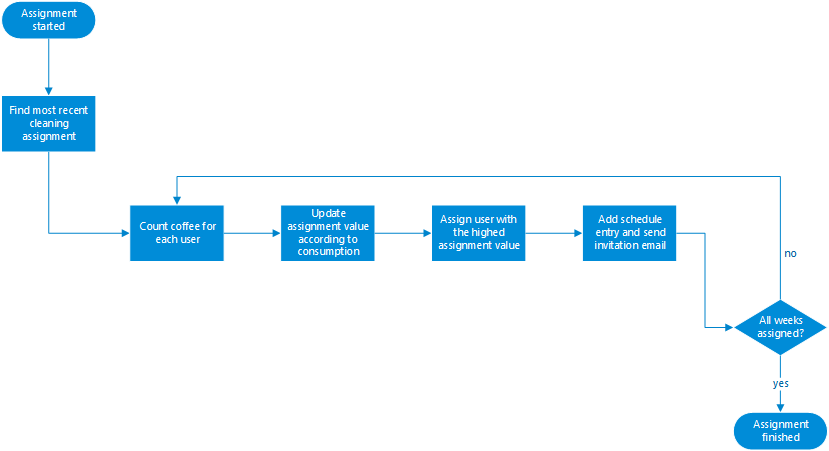
\includegraphics[width=\textwidth]{../images/scheduling.png}}
\caption{priority elevation algorithm}
\end{figure}

\subsection{Coffee pricing}\label{coffee-pricing}

In order to change the price of a single coffee a server administrator
has to change the project configuration which is found in the
\texttt{settings.py} file and alter
the \texttt{COFFEE\_PRICE} setting into the desired value. The default
value is \texttt{0.25} euros.

\begin{lstlisting}[language=python]
COFFEE_PRICE = 0.25
\end{lstlisting}

The price of a double coffee is automatically calculated.

\subsection{Admin interface}\label{admin-interface}

Our application provides an administration interface to manage all
models by hand. It can only be accessed by \emph{staff} users. These
have to be assigned by a server administrator. A staff member can only
manage those models he was given the permissions for.

\begin{figure}[htbp]
\centering
\makebox[\textwidth]{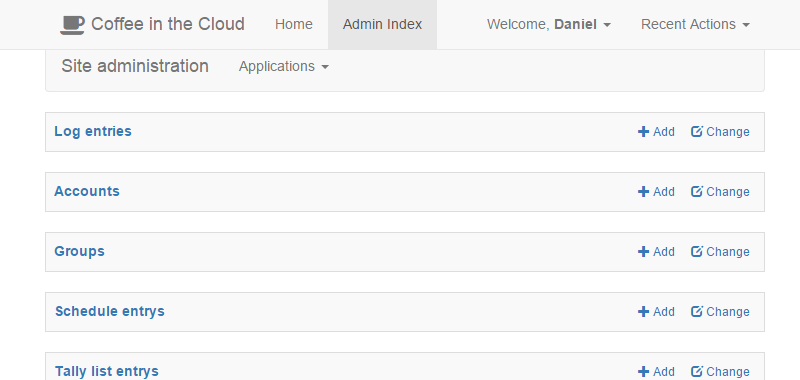
\includegraphics[width=\textwidth]{../images/django-admin.png}}
\caption{default administration view}
\end{figure}

This interface should be used with caution as we provided a frontend
solution for most necessary functionality. Improper changes might
interfere with the platform's integrity.

\subsubsection{Log Entries}\label{log-entries}

Displays a list of administrative events. This can be useful to track
unwanted access and modifications.

\subsubsection{Accounts}\label{accounts}

Displays a list of all available accounts. An administrator can edit
these accounts or create a new one. The account management can also be
used to reset a user's password and to assign permissions or groups.

For every model django provides three different permissions that have to
be assigned:

\begin{description}
\item[add] The user can add a new object.
\item[change] The user can modify an existing object.
\item[delete] The user can remove an existing object from the
database.
\end{description}

As long as a user has access to one of these permissions he will see the
model in his administration interface.

Apart from individually assigning permissions to users it is possible to
assign them to groups. These groups then apply the permissions to the
selected users.

\subsubsection{Groups}\label{groups}

Displays a list of all available groups. It is possible for an
administrator to add new groups or group members.

\subsubsection{Schedule Entries}\label{schedule-entries}

Displays a list of all schedule entries for the cleaning schedule. These
can be manually edited in case a wrong or unwanted assignment occurred.

\subsubsection{Tally List Entries}\label{tally-list-entries}

Displays a list of all tally list entries and their respective users.
These can be added in case a coffee was wrongfully added and the default
deleting time expired.

\newpage
\newpage
\section{Application Setup and
Deployment}\label{application-setup-and-deployment}

In order to deploy our application you will need the following
components installed on your system:

\begin{itemize}
\item
  Python 2.7 including PIP
\item
  Apache including \texttt{mod\_wsgi}
\item
  Node Package Manager (npm)
\item
  Git
\end{itemize}

\subsection{Clone the repository}\label{clone-the-repository}

At first you have to clone the repository from github.

\begin{verbatim}
git clone https://github.com/Birne94/Coffee-in-the-Cloud.git
\end{verbatim}

\subsection{Install client
dependencies}\label{install-client-dependencies}

Install bower and grunt.

\begin{verbatim}
npm -g install bower
npm -g install grunt
npm -g install grunt-cli
\end{verbatim}

Install dependencies and compile less (run inside client directory).

\begin{verbatim}
npm install
bower install
grunt less
\end{verbatim}

\subsection{Install server
dependencies}\label{install-server-dependencies}

Install dependencies and create the database (run inside server
directory).

\begin{verbatim}
python install-dependencies.py
python manage.py migrate
\end{verbatim}

Copy the file \texttt{setup/settings2.py} to \texttt{server/server/} and
adjust \texttt{MEDIA\_ROOT} (absolute path).

Copy the file \texttt{setup/django.wsgi} to \texttt{server/apache/} and
adjust absolute path names.

\subsection{Configure apache}\label{configure-apache}

Add the contents of the file \texttt{setup/apache.conf} to your apache
configuration or include it.

Adjust the port, virtual host and absolute path names for the
application and your local python installation.

\subsection{Adjust permissions}\label{adjust-permissions}

Make the \texttt{server} directory, \texttt{server/db.sqlite3} and
\texttt{server/static/upload/} writable to everyone
(\texttt{chmod\ 777}).

\subsection{Restart apache}\label{restart-apache}

After restarting apache the application should be accessible.

\newpage
\newpage
\section{User manual}\label{user-manual}

\subsection{Tablet}\label{tablet}

When accessing the application through the tablet in the kitchen you
will see a list of users.

\begin{figure}[htbp]
\centering
\makebox[\textwidth]{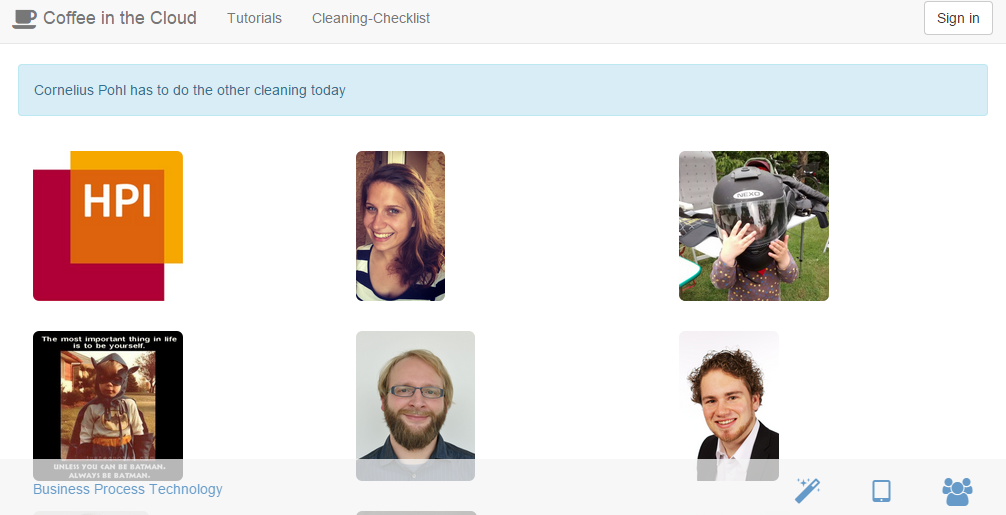
\includegraphics[width=\textwidth]{images/app-tablet-overview.png}}
\caption{tablet screen}
\end{figure}

There you track a coffee without authenticating yourself by tapping on
your profile picture. The list is sorted by the amount of coffee a
person consumed so you might have to scroll down a little bit.

In the following dialog you can select either a single or a double
coffee by tapping on the small (single) or large (double) cup.

In case the kitchen was dirty you can use the \emph{Was the kitchen
dirty?} button to message the person that tracked the most recent
coffee.

\begin{figure}[htbp]
\centering
\makebox[\textwidth]{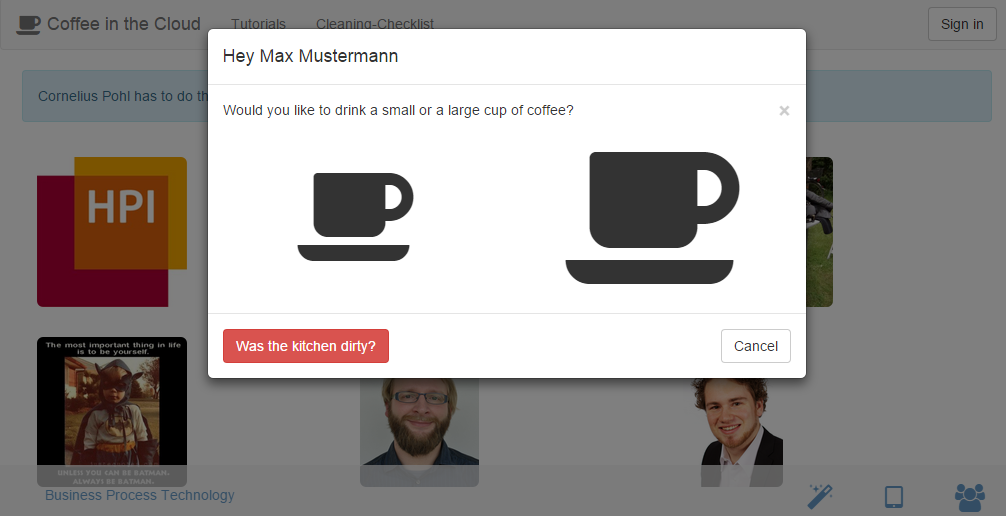
\includegraphics[width=\textwidth]{images/app-tablet-track.png}}
\caption{coffee tracking}
\end{figure}

Afterwards you should see a notification that your coffee has been added
successfully.

\subsection{Tutorials}\label{tutorials-1}

In case you are not familiar with the process of coffee making you can
select the \emph{Tutorials} menu. There you will find a picture tutorial
with each step involved in making coffee.

You can switch to the next step by tapping on the current picture. If
there is a decision to be made, like single/double coffee, you have to
tap on the corresponding picture.

\begin{figure}[htbp]
\centering
\makebox[\textwidth]{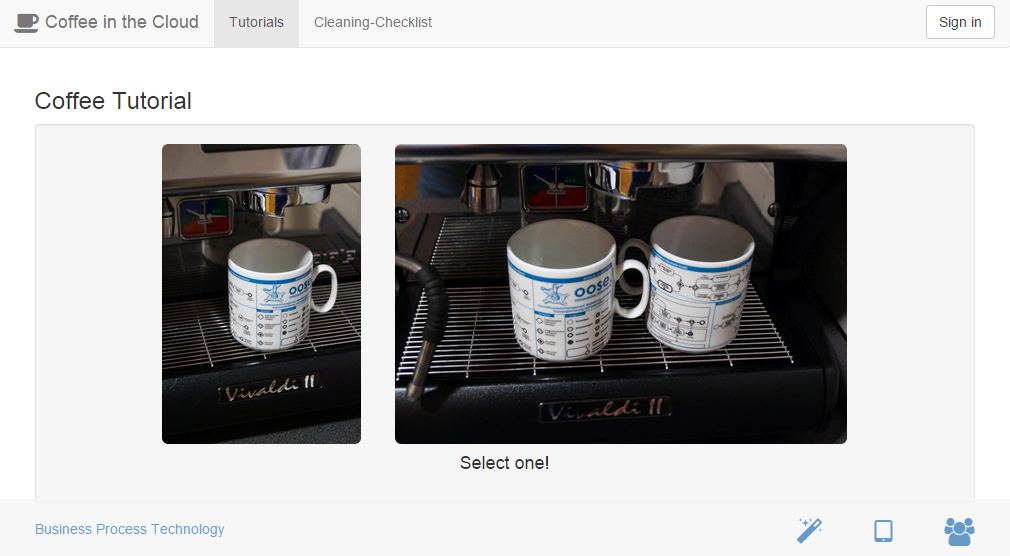
\includegraphics[width=\textwidth]{images/app-tutorial.png}}
\caption{picture tutorial}
\end{figure}

\subsection{Cleaning Checklist}\label{cleaning-checklist-1}

If you are assigned for cleaning you can use the cleaning checklist to
keep track of the necessary steps. By tapping on a step you can mark
them as done. On the bottom you will find a button for resetting the
checklist and marking the cleaning as finished.

\begin{figure}[htbp]
\centering
\makebox[\textwidth]{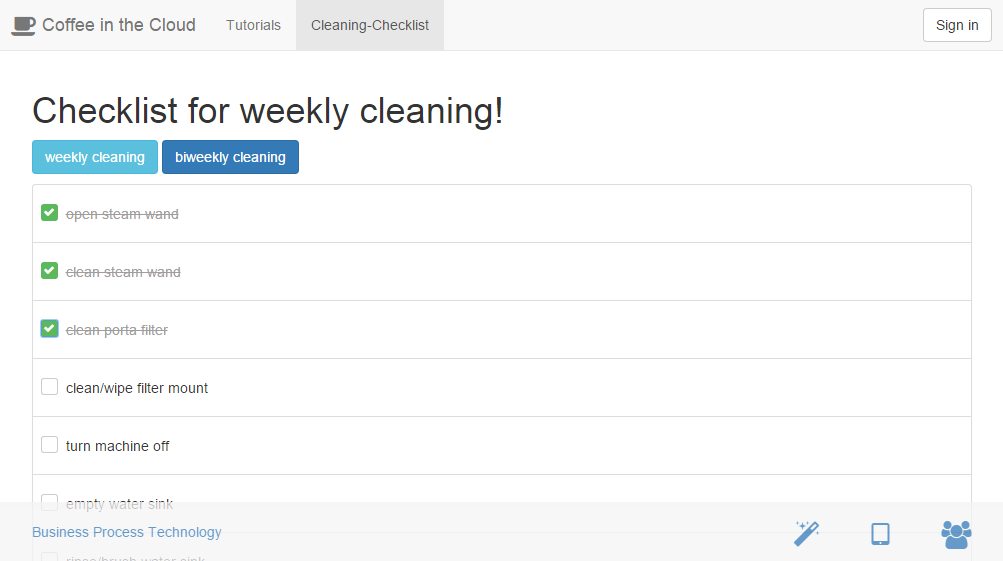
\includegraphics[width=\textwidth]{images/app-checklist.png}}
\caption{cleaning checklist}
\end{figure}

\subsection{Login}\label{login-1}

When accessing the application through your browser you will see a
welcoming screen like this.

\begin{figure}[htbp]
\centering
\makebox[\textwidth]{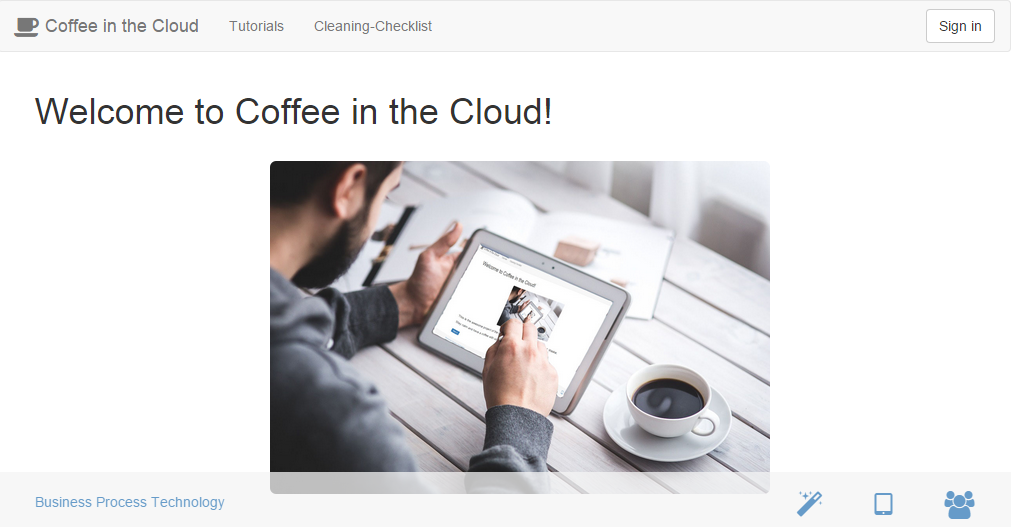
\includegraphics[width=\textwidth]{images/app-welcome.png}}
\caption{welcome screen}
\end{figure}

In the top right corner you can sign in using your email address and
password. These credentials should be provided by a system
administrator.

\begin{figure}[htbp]
\centering
\makebox[\textwidth]{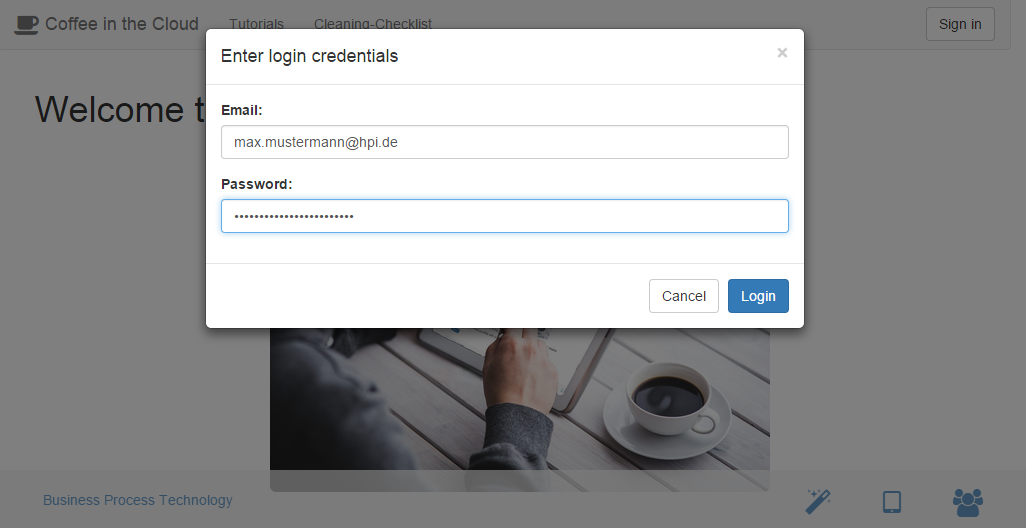
\includegraphics[width=\textwidth]{images/app-login.png}}
\caption{login screen}
\end{figure}

After successfully logging in you will be greeted personally and can see
an overview of your account like the amount of coffees drunk or your
current balance.

\begin{figure}[htbp]
\centering
\makebox[\textwidth]{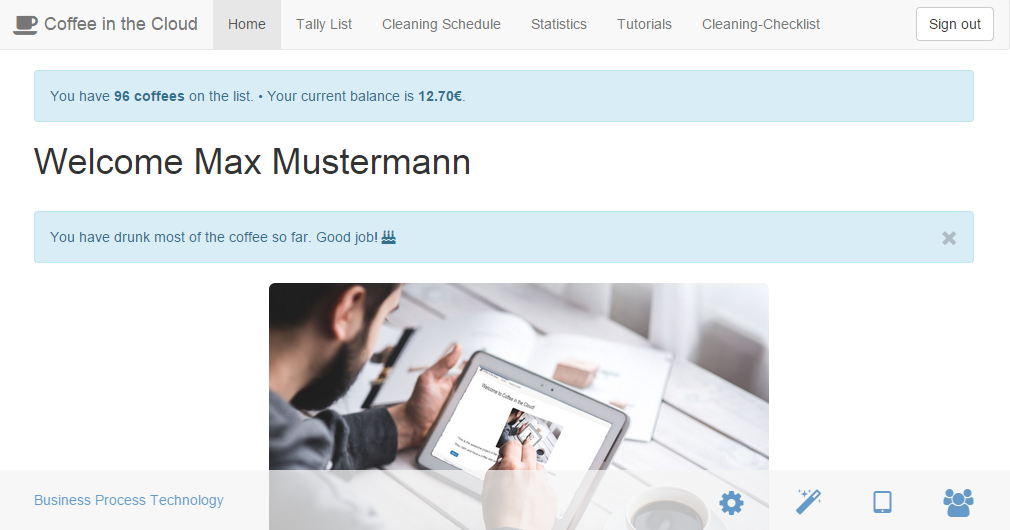
\includegraphics[width=\textwidth]{images/app-welcome-user.png}}
\caption{welcome screen}
\end{figure}

You can now access more modules than before.

\subsection{Tally List}\label{tally-list-1}

The tally list screen gives you an overview of the last ten coffees that
have been added to your account. Apart from that you will see your
current balance.

In case you wrongfully booked a coffee you can remove it by accessing
this page within half an hour.

\begin{figure}[htbp]
\centering
\makebox[\textwidth]{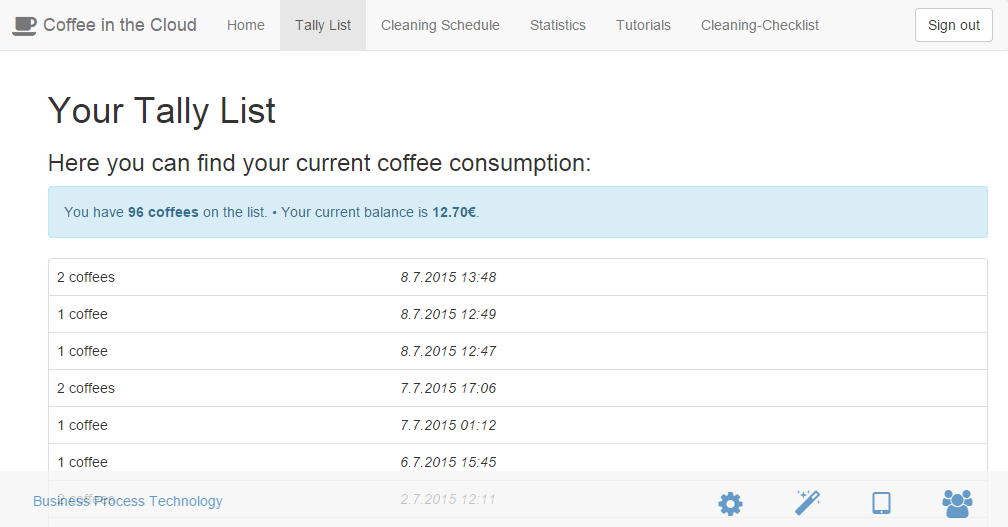
\includegraphics[width=\textwidth]{images/app-tally.png}}
\caption{tally list screen}
\end{figure}

\subsection{Cleaning Schedule}\label{cleaning-schedule-1}

The cleaning schedule shows who is assigned for cleaning the kitchen in
the next weeks. It differentiates between weekly, biweekly and other
cleaning. If a cleaning has successfully been done it will be crossed
out.

If you are assigned for cleaning you will also get a notification and
can mark it as done.

\begin{figure}[htbp]
\centering
\makebox[\textwidth]{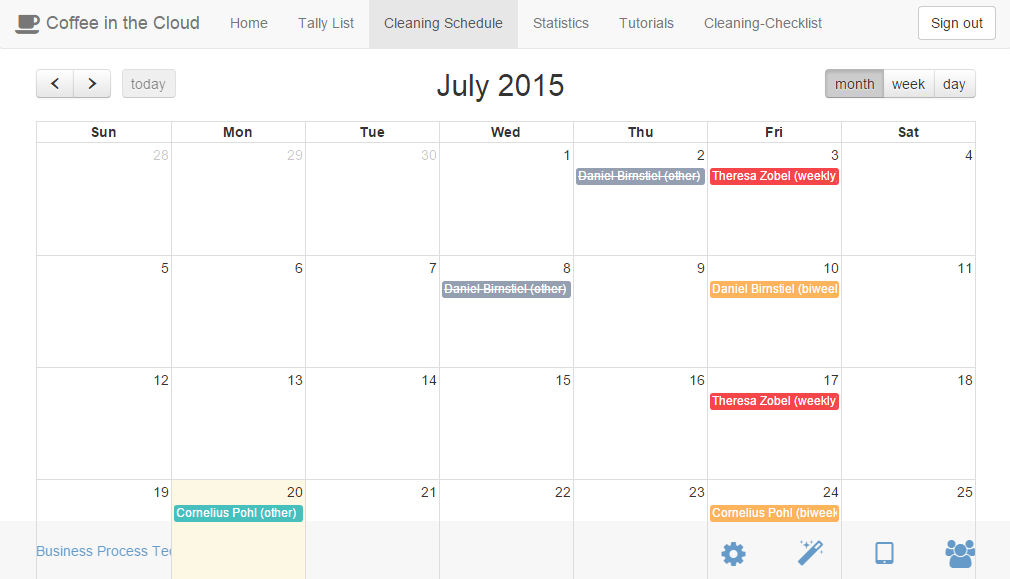
\includegraphics[width=\textwidth]{images/app-schedule.png}}
\caption{cleaning schedule}
\end{figure}

\subsection{Statistics}\label{statistics-2}

In case you wondered how your own coffee consumption changed over time
or how it compares to everyone else you can do so using this page.

\begin{figure}[htbp]
\centering
\makebox[\textwidth]{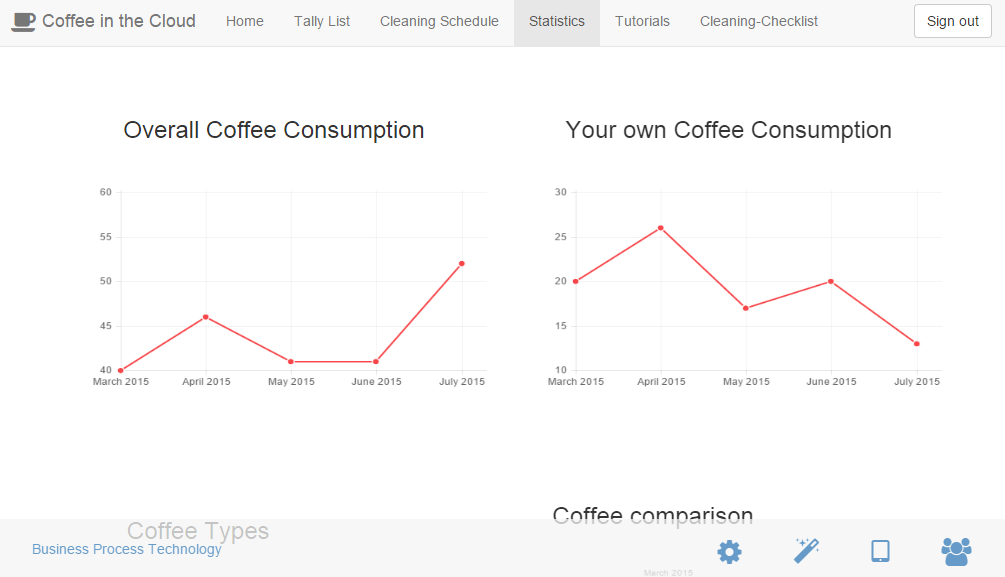
\includegraphics[width=\textwidth]{images/app-statistics.png}}
\caption{statistics screen}
\end{figure}

\subsection{Settings}\label{settings-2}

In the bottom line you will find a gear symbol under which you have the
option to change your account settings.

\begin{figure}[htbp]
\centering
\makebox[\textwidth]{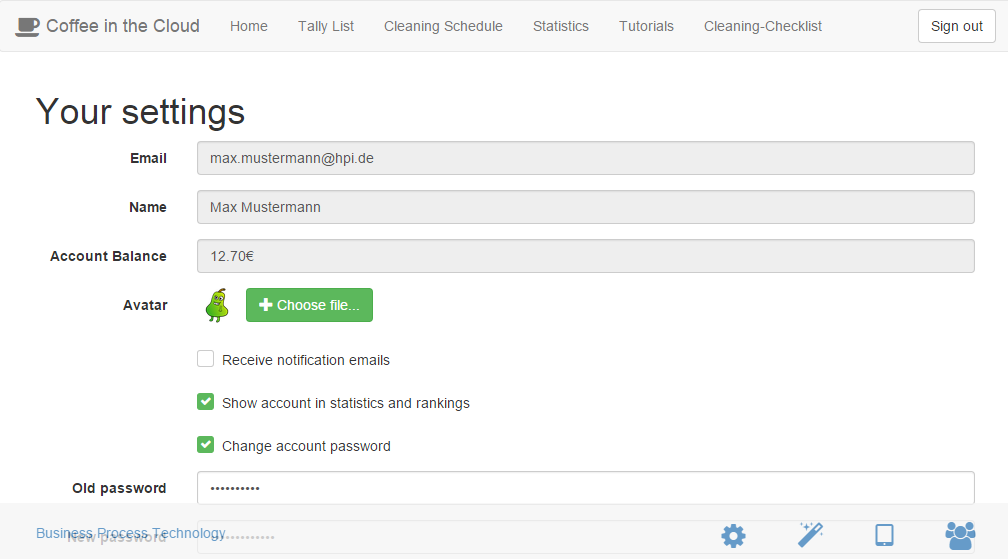
\includegraphics[width=\textwidth]{images/app-settings.png}}
\caption{settings screen}
\end{figure}

In case you have the permission to manage the global balance you can do
that here as well. You can either select a user to update his amount or
update the global balance.

In order to subtract money from the global balance you have to enter a
negative number.

\begin{figure}[htbp]
\centering
\makebox[\textwidth]{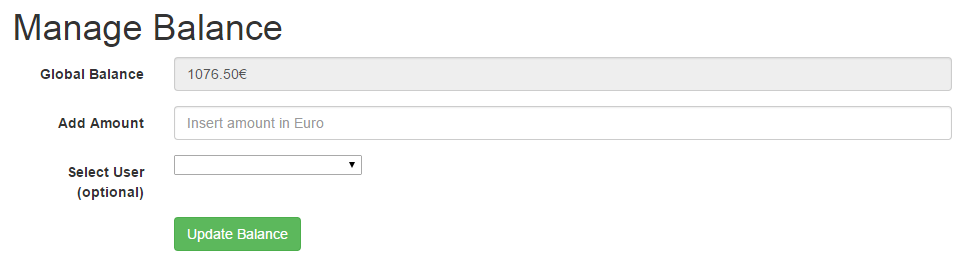
\includegraphics[width=\textwidth]{images/app-balance.png}}
\caption{global balance settings}
\end{figure}

\newpage
\newpage
\section{Conclusion}\label{conclusion}

The main goal was to implement a web application in order to support the
BPT chair at the HPI.

Some core aspects were to have a tally list and and payment balance
as well as the possibility to provide a convenient way to track the users
coffees in the kitchen. This replaces the \emph{old fashioned} tally
list that was used before.

Although we could not achieve all the aspects, like payment options or
automatic ordering, we are proud of the project. During the process of
implementation we were supported optimally by our tutors Marcin,
Adriatik and Rami.

All in all one could say it was a fascinating project with a great team.
We are looking forward to seeing the application in action!

\vspace{2cm}

You can find the project at: \href{https://github.com/Birne94/Coffee-in-the-Cloud}{https://github.com/Birne94/Coffee-in-the-Cloud}.
